
%\documentclass[journal]{IEEEtran}
\documentclass[conference,twoside]{IEEEtran}


\usepackage{cite}
\usepackage{listings}




% *** GRAPHICS RELATED PACKAGES ***
%
\ifCLASSINFOpdf
  \usepackage[pdftex]{graphicx}
  % declare the path(s) where your graphic files are
  \graphicspath{{./images/}}
  % and their extensions so you won't have to specify these with
  % every instance of \includegraphics
  \DeclareGraphicsExtensions{.pdf,.jpeg,.jpg,.png}
  \usepackage{tikz}
  \usetikzlibrary{automata,positioning,trees,chains,decorations.pathreplacing,angles,quotes,angles,arrows}
  \usepackage{adjustbox}
  \usepackage[section]{placeins}
  \usepackage{calc}
\else
  % or other class option (dvipsone, dvipdf, if not using dvips). graphicx
  % will default to the driver specified in the system graphics.cfg if no
  % driver is specified.
  % \usepackage[dvips]{graphicx}
  % declare the path(s) where your graphic files are
  % \graphicspath{{../eps/}}
  % and their extensions so you won't have to specify these with
  % every instance of \includegraphics
  % \DeclareGraphicsExtensions{.eps}
\fi



% *** MATH PACKAGES ***
%
\usepackage{amsmath}
\usepackage{nicefrac}
\interdisplaylinepenalty=2500
% restore such page breaks as IEEEtran.cls normally does





% *** SPECIALIZED LIST PACKAGES ***
%
%\usepackage{algorithmic}
% algorithmic.sty was written by Peter Williams and Rogerio Brito.
% This package provides an algorithmic environment fo describing algorithms.
% You can use the algorithmic environment in-text or within a figure
% environment to provide for a floating algorithm. Do NOT use the algorithm
% floating environment provided by algorithm.sty (by the same authors) or
% algorithm2e.sty (by Christophe Fiorio) as the IEEE does not use dedicated
% algorithm float types and packages that provide these will not provide
% correct IEEE style captions. The latest version and documentation of
% algorithmic.sty can be obtained at:
% http://www.ctan.org/pkg/algorithms
% Also of interest may be the (relatively newer and more customizable)
% algorithmicx.sty package by Szasz Janos:
% http://www.ctan.org/pkg/algorithmicx




% *** ALIGNMENT PACKAGES ***
%
\usepackage{array}
% Frank Mittelbach's and David Carlisle's array.sty patches and improves
% the standard LaTeX2e array and tabular environments to provide better
% appearance and additional user controls. As the default LaTeX2e table
% generation code is lacking to the point of almost being broken with
% respect to the quality of the end results, all users are strongly
% advised to use an enhanced (at the very least that provided by array.sty)
% set of table tools. array.sty is already installed on most systems. The
% latest version and documentation can be obtained at:
% http://www.ctan.org/pkg/array


% IEEEtran contains the IEEEeqnarray family of commands that can be used to
% generate multiline equations as well as matrices, tables, etc., of high
% quality.




% *** SUBFIGURE PACKAGES ***
%\ifCLASSOPTIONcompsoc
%  \usepackage[caption=false,font=normalsize,labelfont=sf,textfont=sf]{subfig}
%\else
%  \usepackage[caption=false,font=footnotesize]{subfig}
%\fi
% subfig.sty, written by Steven Douglas Cochran, is the modern replacement
% for subfigure.sty, the latter of which is no longer maintained and is
% incompatible with some LaTeX packages including fixltx2e. However,
% subfig.sty requires and automatically loads Axel Sommerfeldt's caption.sty
% which will override IEEEtran.cls' handling of captions and this will result
% in non-IEEE style figure/table captions. To prevent this problem, be sure
% and invoke subfig.sty's "caption=false" package option (available since
% subfig.sty version 1.3, 2005/06/28) as this is will preserve IEEEtran.cls
% handling of captions.
% Note that the Computer Society format requires a larger sans serif font
% than the serif footnote size font used in traditional IEEE formatting
% and thus the need to invoke different subfig.sty package options depending
% on whether compsoc mode has been enabled.
%
% The latest version and documentation of subfig.sty can be obtained at:
% http://www.ctan.org/pkg/subfig




% *** FLOAT PACKAGES ***
%
%\usepackage{fixltx2e}
% fixltx2e, the successor to the earlier fix2col.sty, was written by
% Frank Mittelbach and David Carlisle. This package corrects a few problems
% in the LaTeX2e kernel, the most notable of which is that in current
% LaTeX2e releases, the ordering of single and double column floats is not
% guaranteed to be preserved. Thus, an unpatched LaTeX2e can allow a
% single column figure to be placed prior to an earlier double column
% figure.
% Be aware that LaTeX2e kernels dated 2015 and later have fixltx2e.sty's
% corrections already built into the system in which case a warning will
% be issued if an attempt is made to load fixltx2e.sty as it is no longer
% needed.
% The latest version and documentation can be found at:
% http://www.ctan.org/pkg/fixltx2e


%\usepackage{stfloats}
% stfloats.sty was written by Sigitas Tolusis. This package gives LaTeX2e
% the ability to do double column floats at the bottom of the page as well
% as the top. (e.g., "\begin{figure*}[!b]" is not normally possible in
% LaTeX2e). It also provides a command:
%\fnbelowfloat
% to enable the placement of footnotes below bottom floats (the standard
% LaTeX2e kernel puts them above bottom floats). This is an invasive package
% which rewrites many portions of the LaTeX2e float routines. It may not work
% with other packages that modify the LaTeX2e float routines. The latest
% version and documentation can be obtained at:
% http://www.ctan.org/pkg/stfloats
% Do not use the stfloats baselinefloat ability as the IEEE does not allow
% \baselineskip to stretch. Authors submitting work to the IEEE should note
% that the IEEE rarely uses double column equations and that authors should try
% to avoid such use. Do not be tempted to use the cuted.sty or midfloat.sty
% packages (also by Sigitas Tolusis) as the IEEE does not format its papers in
% such ways.
% Do not attempt to use stfloats with fixltx2e as they are incompatible.
% Instead, use Morten Hogholm'a dblfloatfix which combines the features
% of both fixltx2e and stfloats:
%
\usepackage{dblfloatfix}
% The latest version can be found at:
% http://www.ctan.org/pkg/dblfloatfix




%\ifCLASSOPTIONcaptionsoff
%  \usepackage[nomarkers]{endfloat}
% \let\MYoriglatexcaption\caption
% \renewcommand{\caption}[2][\relax]{\MYoriglatexcaption[#2]{#2}}
%\fi
% endfloat.sty was written by James Darrell McCauley, Jeff Goldberg and
% Axel Sommerfeldt. This package may be useful when used in conjunction with
% IEEEtran.cls'  captionsoff option. Some IEEE journals/societies require that
% submissions have lists of figures/tables at the end of the paper and that
% figures/tables without any captions are placed on a page by themselves at
% the end of the document. If needed, the draftcls IEEEtran class option or
% \CLASSINPUTbaselinestretch interface can be used to increase the line
% spacing as well. Be sure and use the nomarkers option of endfloat to
% prevent endfloat from "marking" where the figures would have been placed
% in the text. The two hack lines of code above are a slight modification of
% that suggested by in the endfloat docs (section 8.4.1) to ensure that
% the full captions always appear in the list of figures/tables - even if
% the user used the short optional argument of \caption[]{}.
% IEEE papers do not typically make use of \caption[]'s optional argument,
% so this should not be an issue. A similar trick can be used to disable
% captions of packages such as subfig.sty that lack options to turn off
% the subcaptions:
% For subfig.sty:
% \let\MYorigsubfloat\subfloat
% \renewcommand{\subfloat}[2][\relax]{\MYorigsubfloat[]{#2}}
% However, the above trick will not work if both optional arguments of
% the \subfloat command are used. Furthermore, there needs to be a
% description of each subfigure *somewhere* and endfloat does not add
% subfigure captions to its list of figures. Thus, the best approach is to
% avoid the use of subfigure captions (many IEEE journals avoid them anyway)
% and instead reference/explain all the subfigures within the main caption.
% The latest version of endfloat.sty and its documentation can obtained at:
% http://www.ctan.org/pkg/endfloat
%
% The IEEEtran \ifCLASSOPTIONcaptionsoff conditional can also be used
% later in the document, say, to conditionally put the References on a
% page by themselves.


\usepackage{url}

% correct bad hyphenation here
\hyphenation{op-tical net-works semi-conduc-tor}

\usepackage{textcomp}

\newcommand{\lref}[1]{(Listing \ref{#1} on page \pageref{#1})}
\newcommand{\eref}[1]{(\ref{#1})}
\newcommand{\fref}[1]{Figure \ref{#1}}
\newcommand{\sref}[1]{Section \ref{#1}}
\newcommand{\code}[1]{\texttt{#1}}

\title{Transforming and Caching Entries from Massive, Online Databases using Apache Spark and MongoDB}
%\author{Mark~McDermott, \\ Student~MS.~E.E., George~Mason~University \\ mmcderm1@gmu.edu}
\author{
\IEEEauthorblockN{Mark E. McDermott} \\
\IEEEauthorblockA{Volgenau School of Engineering\\
George Mason University\\
Fairfax, VA 22030\\
Email: mmcderm1@gmu.edu} \\
\and
\IEEEauthorblockN{Jose A. Velasquez-Principe} \\
\IEEEauthorblockA{Volgenau School of Engineering\\
George Mason University\\
Fairfax, VA 22030\\
Email: jvelasq@gmu.edu}
}

\lstdefinelanguage{Txt}
{
    basicstyle=\ttfamily\small,
    keepspaces=true,
    columns=fullflexible,
    frame=single,
}

\makeatletter
\def\lst@makecaption{%
  \def\@captype{table}%
  \@makecaption
}
\makeatother



\begin{document}
% The paper headers
\markboth{ECE 499/590 Big Data Technologies, George Mason University, May~2020}%
{Final Project}

% make the title area
\maketitle


\begin{abstract}
Online databases with user generated content are increasingly common. If the number of users of such a database is large then the amount of content can quickly grow to be very large. This means that it is impractical and expensive to allow users to access the database in its entirety. To work around this many sites provide feature-rich search and query APIs that allow users to download only the portions of the database that they require. After downloading the data the users then processes it using their local computing resources. A very common operation to be performed by users is to perform preprocessing and cleaning of the data since, due the distributed sources of the data, it is likely to be of varying quality. This represents duplication of work that could be captured back into the public database. We present an architecture based on Apache Spark for performing this cleanup near the source of the data. We also present the creation of a cache of cleaned data so that other users can benefit from the work and analysis already performed. We demonstrate its effectiveness using a real-world example: We perform spectral filtering of recordings from the Xeno Canto database of bird-songs and then cache the filtered results.
\end{abstract}

% Note that keywords are not normally used for peerreview papers.
%\begin{IEEEkeywords}
%Beamformer, MVDR, MPDR, Mismatch
%\end{IEEEkeywords}



% For peer review papers, you can put extra information on the cover
% page as needed:
% \ifCLASSOPTIONpeerreview
% \begin{center} \bfseries EDICS Category: 3-BBND \end{center}
% \fi
%
% For peerreview papers, this IEEEtran command inserts a page break and
% creates the second title. It will be ignored for other modes.
\IEEEpeerreviewmaketitle




%%%%%%%%%%%%%%%%%%%%%%%%%%%%%%%%%%%%%%%%%%%%%%%%%%%%%%%%%%%%%%%%%%%%%%%%%%%%%%%%%%%%%%%%%
%%%%%%%%%%%%%%%%%%%%%%%%%%%%%%%%%%%%%%%%%%%%%%%%%%%%%%%%%%%%%%%%%%%%%%%%%%%%%%%%%%%%%%%%%
%%%%%%%%%%%%%%%%%%%%%%%%%%%%%%%%%%%%%%%%%%%%%%%%%%%%%%%%%%%%%%%%%%%%%%%%%%%%%%%%%%%%%%%%%
%%%%%%%%%%%%%%%%%%%%%%%%%%%%%%%%%%%%%%%%%%%%%%%%%%%%%%%%%%%%%%%%%%%%%%%%%%%%%%%%%%%%%%%%%
%%%%%%%%%%%%%%%%%%%%%%%%%%%%%%%%%%%%%%%%%%%%%%%%%%%%%%%%%%%%%%%%%%%%%%%%%%%%%%%%%%%%%%%%%
%%%%%%%%%%%%%%%%%%%%%%%%%%%%%%%%%%%%%%%%%%%%%%%%%%%%%%%%%%%%%%%%%%%%%%%%%%%%%%%%%%%%%%%%%
%%%%%%%%%%%%%%%%%%%%%%%%%%%%%%%%%%%%%%%%%%%%%%%%%%%%%%%%%%%%%%%%%%%%%%%%%%%%%%%%%%%%%%%%%
%%%%%%%%%%%%%%%%%%%%%%%%%%%%%%%%%%%%%%%%%%%%%%%%%%%%%%%%%%%%%%%%%%%%%%%%%%%%%%%%%%%%%%%%%
\section{Introduction}
% The very first letter is a 2 line initial drop letter followed
% by the rest of the first word in caps.
%
% form to use if the first word consists of a single letter:
% \IEEEPARstart{A}{demo} file is ....
%
% form to use if you need the single drop letter followed by
% normal text (unknown if ever used by the IEEE):
% \IEEEPARstart{A}{}demo file is ....
%
% Some journals put the first two words in caps:
% \IEEEPARstart{T}{his demo} file is ....
%
% Here we have the typical use of a "T" for an initial drop letter
% and "HIS" in caps to complete the first word.
\IEEEPARstart{O}{ne} very interesting development to come from the cloud computing and data science explosion is crowd sourced data bases. These databases can grow very large as the work it takes to curate the databases is distributed around the globe. This distributed nature presents some challenges though.

One issue is that quality of individual entries in a database can vary since no single source or curator was involved in generating the entries. Some data providers, such as Kaggle\cite{kaggle}, solve this by allowing users to rate the quality of datasets. However this approach, while it does provide useful information to potential users, does not do anything to improve quality. A dataset uploaded to a service such as Kaggle can only be updated by the user that uploaded it so improving the quality of a dataset after it is created can only be done by the original user. This reduces the benefits of distributed data curation.

Another challenge is that the meta data associated with particular data points can vary greatly based on the individual contributor's capacity to gather the data. This could be solved by careful curation of the submissions to ensure that each data point is properly labeled with metadata but this again reduces the benefits of crowd sourcing data collection.

We found a particular example on Kaggle that highlights this issue and inspired this project. A user of the very large, user generated database of bird call recordings - Xeno Cano\cite{xenocanto} - uploaded a carefully curated subset of the Xeno Canto library to Kaggle so that it was ready for data science workflows\cite{xenocantokaggle}. This represents significant work that would have to duplicated in the future since the Xeno Canto database continues to grow as user's submit new recordings. The recordings are of many different lengths and have different levels of background noise, thus necessitating the cleanup step prior to use for data science.
%%Jose

In this paper we present an architecture that allows for crowd sourcing the curation efforts by caching cleaned up data points using a database based on flexible schema. This allows user's to perform the necessary data manipulation efforts and save the results for other's to use without requiring updating the source database's schema. We pair this cache with Apache Spark to allow for distributed processing of user's requests.


%%%%%%%%%%%%%%%%%%%%%%%%%%%%%%%%%%%%%%%%%%%%%%%%%%%%%%%%%%%%%%%%%%%%%%%%%%%%%%%%%%%%%%%%%
%%%%%%%%%%%%%%%%%%%%%%%%%%%%%%%%%%%%%%%%%%%%%%%%%%%%%%%%%%%%%%%%%%%%%%%%%%%%%%%%%%%%%%%%%
%%%%%%%%%%%%%%%%%%%%%%%%%%%%%%%%%%%%%%%%%%%%%%%%%%%%%%%%%%%%%%%%%%%%%%%%%%%%%%%%%%%%%%%%%
%%%%%%%%%%%%%%%%%%%%%%%%%%%%%%%%%%%%%%%%%%%%%%%%%%%%%%%%%%%%%%%%%%%%%%%%%%%%%%%%%%%%%%%%%
%%%%%%%%%%%%%%%%%%%%%%%%%%%%%%%%%%%%%%%%%%%%%%%%%%%%%%%%%%%%%%%%%%%%%%%%%%%%%%%%%%%%%%%%%
%%%%%%%%%%%%%%%%%%%%%%%%%%%%%%%%%%%%%%%%%%%%%%%%%%%%%%%%%%%%%%%%%%%%%%%%%%%%%%%%%%%%%%%%%
%%%%%%%%%%%%%%%%%%%%%%%%%%%%%%%%%%%%%%%%%%%%%%%%%%%%%%%%%%%%%%%%%%%%%%%%%%%%%%%%%%%%%%%%%
%%%%%%%%%%%%%%%%%%%%%%%%%%%%%%%%%%%%%%%%%%%%%%%%%%%%%%%%%%%%%%%%%%%%%%%%%%%%%%%%%%%%%%%%%
\section{Technology Stack}
Figure \ref{fig:tech} shows the technologies we integrated for this project, each of which is introduced in this section. In the next section we show in detail how these technologies can be used together to create a cache of the Xeno Canto database.
\begin{figure*}[tb]  %image placeholder
  \centering
  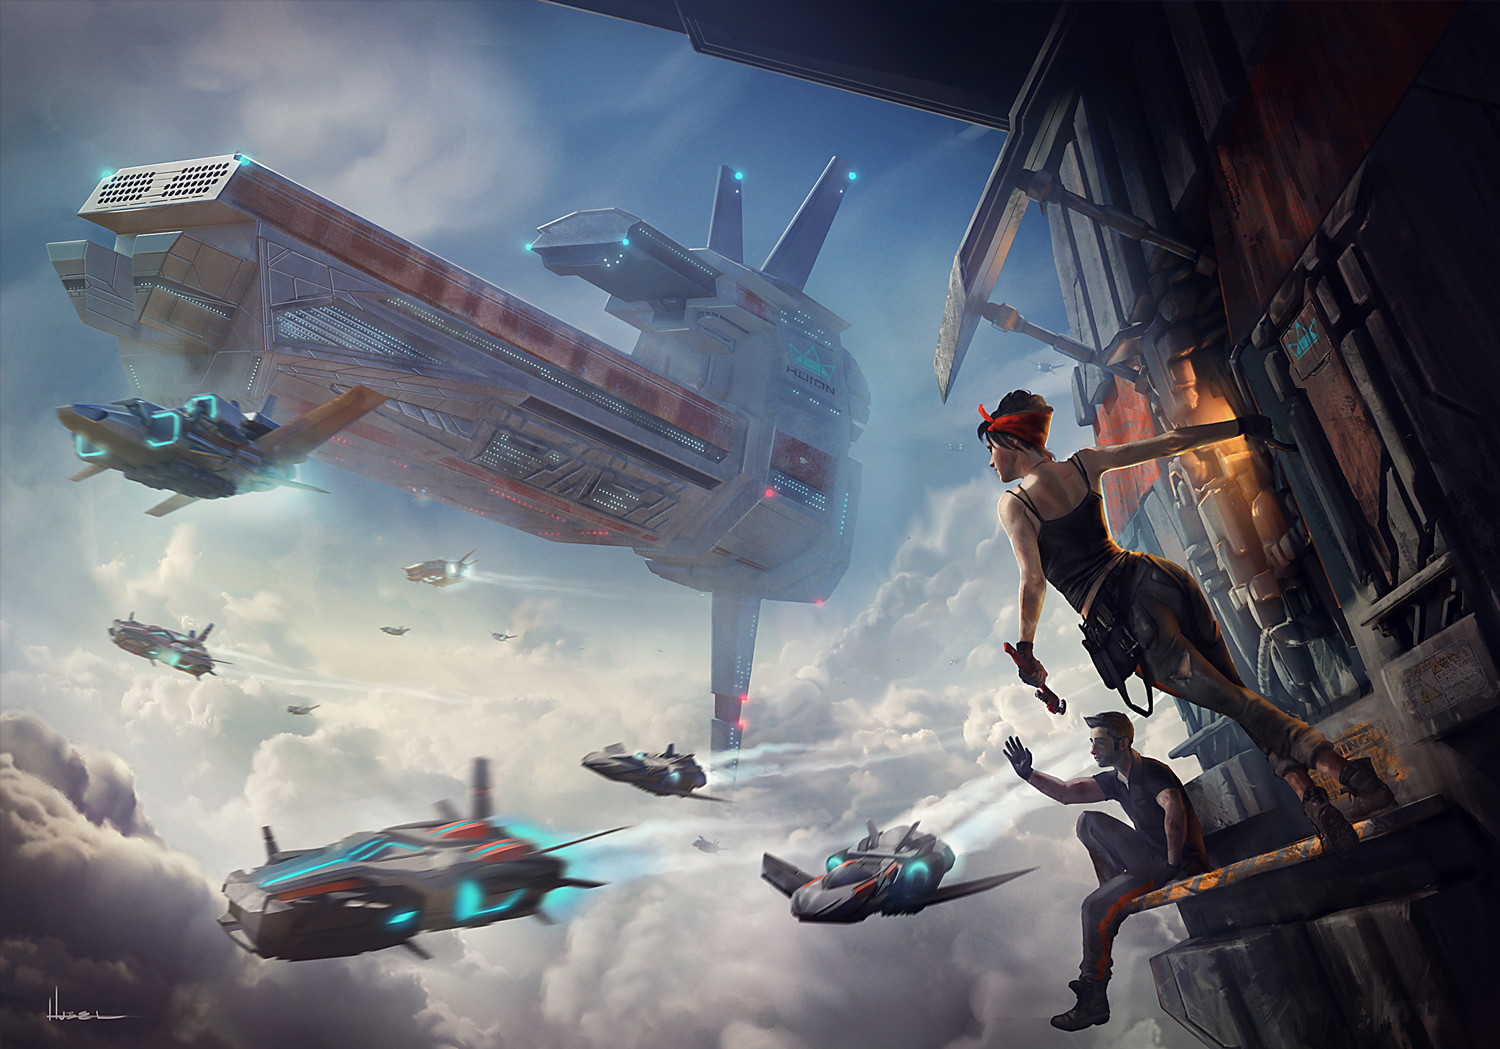
\includegraphics[width=\textwidth]{tech_stack}
  \caption{Technology stack used in this project.}
  \label{fig:tech}
\end{figure*}


%%%%%%%%%%%%%%%%%%%%%%%%%%%%%%%%%%%%%%%%%%%%%%%%%%%%%%%%%%%%%%%%%%%%%%%%%%%%%%%%%%%%%%%%%
%%%%%%%%%%%%%%%%%%%%%%%%%%%%%%%%%%%%%%%%%%%%%%%%%%%%%%%%%%%%%%%%%%%%%%%%%%%%%%%%%%%%%%%%%
%%%%%%%%%%%%%%%%%%%%%%%%%%%%%%%%%%%%%%%%%%%%%%%%%%%%%%%%%%%%%%%%%%%%%%%%%%%%%%%%%%%%%%%%%
%%%%%%%%%%%%%%%%%%%%%%%%%%%%%%%%%%%%%%%%%%%%%%%%%%%%%%%%%%%%%%%%%%%%%%%%%%%%%%%%%%%%%%%%%
\subsection{MongoDB \& MongoDB Compass}
MongoDB is a cross-platform program that allow users to create databases for very large data and is used in an abundance of modern applications. MongoDB differs from traditional SQL databases in that data is stored as JSON documents with a flexible schema. This is crucial in applications where data comes from diverse sources and may be of differing quality and completeness. Because each entry in MongoDB is stored as a JSON document MongoDB pairs naturaly with internet APIs where JSON is the defacto format for transfering data. MongoDB can handle very large files with millions of records of data with ease\cite{mongodb}.

MongoDB Compass is a freely available desktop application for Linux, Mac, and Microsoft Windows that allows viewing and editing of remote MongoDB databases. This tool also allows for engineers to view read/write performance statistics to help them resolve performance issues\cite{mongodbcompass}.

%%%%%%%%%%%%%%%%%%%%%%%%%%%%%%%%%%%%%%%%%%%%%%%%%%%%%%%%%%%%%%%%%%%%%%%%%%%%%%%%%%%%%%%%%
%%%%%%%%%%%%%%%%%%%%%%%%%%%%%%%%%%%%%%%%%%%%%%%%%%%%%%%%%%%%%%%%%%%%%%%%%%%%%%%%%%%%%%%%%
%%%%%%%%%%%%%%%%%%%%%%%%%%%%%%%%%%%%%%%%%%%%%%%%%%%%%%%%%%%%%%%%%%%%%%%%%%%%%%%%%%%%%%%%%
%%%%%%%%%%%%%%%%%%%%%%%%%%%%%%%%%%%%%%%%%%%%%%%%%%%%%%%%%%%%%%%%%%%%%%%%%%%%%%%%%%%%%%%%%
\subsection{Apache Spark}
Apache Spark is a data processing framework that allows users to perform operations on data sets that are very large. Apache Spark is a key application that allows big data and machine learning to be incorporated in a user-friendly application. Spark provides a framework whereby operations on very large data sets can be parallelized and distributed across a cluster of compute resources. Often compared to the earlier technology - Hadoop MapReduce - Spark is 100 times faster for some workloads.

Spark has interfaces in in many popular programming languages. Of particular interest for us is Python which is widely used in the scientific computing community for signal processing and machine learning. Apache Spark allows for user defined functions which enables the whole range of Python based scientific computing libraries to be parallelized on the Spark cluster\cite{spark}.


%%%%%%%%%%%%%%%%%%%%%%%%%%%%%%%%%%%%%%%%%%%%%%%%%%%%%%%%%%%%%%%%%%%%%%%%%%%%%%%%%%%%%%%%%
%%%%%%%%%%%%%%%%%%%%%%%%%%%%%%%%%%%%%%%%%%%%%%%%%%%%%%%%%%%%%%%%%%%%%%%%%%%%%%%%%%%%%%%%%
%%%%%%%%%%%%%%%%%%%%%%%%%%%%%%%%%%%%%%%%%%%%%%%%%%%%%%%%%%%%%%%%%%%%%%%%%%%%%%%%%%%%%%%%%
%%%%%%%%%%%%%%%%%%%%%%%%%%%%%%%%%%%%%%%%%%%%%%%%%%%%%%%%%%%%%%%%%%%%%%%%%%%%%%%%%%%%%%%%%
\subsection{Python}
Python is one the fastest growing programming language\cite{python}. Though considered to be a general purpose language, it has been adopted by the scientific computing community because of the availablity of libraries such as \code{numpy}, \code{scipy}, and \code{matplotlib}. It has also positioned itself as the leader in machine learning applications through the availabilty of high quality machine learning libraries such as \code{tensorflow}, and many others.

Python allows for seamless integration of all technologies to be used in this project since each of the technologies we selected have high quality Python APIs.

%%%%%%%%%%%%%%%%%%%%%%%%%%%%%%%%%%%%%%%%%%%%%%%%%%%%%%%%%%%%%%%%%%%%%%%%%%%%%%%%%%%%%%%%%
%%%%%%%%%%%%%%%%%%%%%%%%%%%%%%%%%%%%%%%%%%%%%%%%%%%%%%%%%%%%%%%%%%%%%%%%%%%%%%%%%%%%%%%%%
%%%%%%%%%%%%%%%%%%%%%%%%%%%%%%%%%%%%%%%%%%%%%%%%%%%%%%%%%%%%%%%%%%%%%%%%%%%%%%%%%%%%%%%%%
%%%%%%%%%%%%%%%%%%%%%%%%%%%%%%%%%%%%%%%%%%%%%%%%%%%%%%%%%%%%%%%%%%%%%%%%%%%%%%%%%%%%%%%%%
\subsection{Jupyter Notebooks}
Jupyter Notebooks is a user-friendly open source application that operates as a GUI or "Notebook App" that allows users to write code similar to a text-editor but results of computation are presented inline with the code\cite{jupyter}. The Juypter Notebook allows us to demonstrate step by step how our architecture is to be used and incorporated for a particular problem domain.


%%%%%%%%%%%%%%%%%%%%%%%%%%%%%%%%%%%%%%%%%%%%%%%%%%%%%%%%%%%%%%%%%%%%%%%%%%%%%%%%%%%%%%%%%
%%%%%%%%%%%%%%%%%%%%%%%%%%%%%%%%%%%%%%%%%%%%%%%%%%%%%%%%%%%%%%%%%%%%%%%%%%%%%%%%%%%%%%%%%
%%%%%%%%%%%%%%%%%%%%%%%%%%%%%%%%%%%%%%%%%%%%%%%%%%%%%%%%%%%%%%%%%%%%%%%%%%%%%%%%%%%%%%%%%
%%%%%%%%%%%%%%%%%%%%%%%%%%%%%%%%%%%%%%%%%%%%%%%%%%%%%%%%%%%%%%%%%%%%%%%%%%%%%%%%%%%%%%%%%
\subsection{OCI Containers}
The Open Container Initiative (OCI) provides standards and formats for containerized computing technologies to ensure compatility of a wide range of products - both commercial and open source\cite{OCI}. We used the container runtime system Podman\cite{rhelpodman} to build and integrate the technologies mentioned above. Containers are a powerful way to automate installation and configuration of software and help unlock automated deployment of cloud services\cite{gartnercontainer}.

In this project we use a container definition to control how all of the components are installed and configured to talk together. The container definition allows for managing each configuration change in a source control system so that we can track changes to configuration over time.

The container is also easily transfered to virtual machines running in the cloud so that efforts to configure and integrate the technologies don't have to be duplicated each time a cloud instance is brought online.

%%%%%%%%%%%%%%%%%%%%%%%%%%%%%%%%%%%%%%%%%%%%%%%%%%%%%%%%%%%%%%%%%%%%%%%%%%%%%%%%%%%%%%%%%
%%%%%%%%%%%%%%%%%%%%%%%%%%%%%%%%%%%%%%%%%%%%%%%%%%%%%%%%%%%%%%%%%%%%%%%%%%%%%%%%%%%%%%%%%
%%%%%%%%%%%%%%%%%%%%%%%%%%%%%%%%%%%%%%%%%%%%%%%%%%%%%%%%%%%%%%%%%%%%%%%%%%%%%%%%%%%%%%%%%
%%%%%%%%%%%%%%%%%%%%%%%%%%%%%%%%%%%%%%%%%%%%%%%%%%%%%%%%%%%%%%%%%%%%%%%%%%%%%%%%%%%%%%%%%
\subsection{Microsoft Azure}
Microsoft Azure is a subscription based application that allows users to create virtual machines (VM). VMs hosted on Microsoft's cloud infrastructure allow running very large and intensive applications that scale horizontally as user's needs increase or decrease. Azure provides tools for managing both large and small clusters of virtual machines across the cloud\cite{azure}.


%%%%%%%%%%%%%%%%%%%%%%%%%%%%%%%%%%%%%%%%%%%%%%%%%%%%%%%%%%%%%%%%%%%%%%%%%%%%%%%%%%%%%%%%%
%%%%%%%%%%%%%%%%%%%%%%%%%%%%%%%%%%%%%%%%%%%%%%%%%%%%%%%%%%%%%%%%%%%%%%%%%%%%%%%%%%%%%%%%%
%%%%%%%%%%%%%%%%%%%%%%%%%%%%%%%%%%%%%%%%%%%%%%%%%%%%%%%%%%%%%%%%%%%%%%%%%%%%%%%%%%%%%%%%%
%%%%%%%%%%%%%%%%%%%%%%%%%%%%%%%%%%%%%%%%%%%%%%%%%%%%%%%%%%%%%%%%%%%%%%%%%%%%%%%%%%%%%%%%%
%%%%%%%%%%%%%%%%%%%%%%%%%%%%%%%%%%%%%%%%%%%%%%%%%%%%%%%%%%%%%%%%%%%%%%%%%%%%%%%%%%%%%%%%%
%%%%%%%%%%%%%%%%%%%%%%%%%%%%%%%%%%%%%%%%%%%%%%%%%%%%%%%%%%%%%%%%%%%%%%%%%%%%%%%%%%%%%%%%%
%%%%%%%%%%%%%%%%%%%%%%%%%%%%%%%%%%%%%%%%%%%%%%%%%%%%%%%%%%%%%%%%%%%%%%%%%%%%%%%%%%%%%%%%%
%%%%%%%%%%%%%%%%%%%%%%%%%%%%%%%%%%%%%%%%%%%%%%%%%%%%%%%%%%%%%%%%%%%%%%%%%%%%%%%%%%%%%%%%%
\section{Architecture}
The previously mentioned technology stack is all the applications needed to complete the task at hand. Thankfully all the applications used were easily incorporated onto each other because of there design and layout. In this section we will explain how these application were incorporated into each other and how these applications collaborate together.

Starting with the virtual machine that was created with the help of Microsoft Azure, allowed for the platform to be created and a base to begin using these other application. Secondly the Podman that are containers that allow these applications to be runned in the background . Also allows these applications to runned seamlessly, because all these application can be launched though a command prompt. Furthermore the database was created with MongoDB because MongoDB is a user-friendly application that works seamlessly with Apache Spark to cache and query to a very large database as needed. Next the Apache Spark is used because this allows the data to be manipulated because Apache Spark is a efficient way to process large data sets, and consequently allowing for greater manipulation of the data. Which is where Juypter Notebook comes in as both a text editor and compiler for all these applications as it supports them and is a user-friendly GUI. Finally Python, Numpy, and Matplotlib are libraries were these manipulations can be done with processes that are pre-built and user defined functions to manipulate the data.

%%%%%%%%%%%%%%%%%%%%%%%%%%%%%%%%%%%%%%%%%%%%%%%%%%%%%%%%%%%%%%%%%%%%%%%%%%%%%%%%%%%%%%%%%
%%%%%%%%%%%%%%%%%%%%%%%%%%%%%%%%%%%%%%%%%%%%%%%%%%%%%%%%%%%%%%%%%%%%%%%%%%%%%%%%%%%%%%%%%
%%%%%%%%%%%%%%%%%%%%%%%%%%%%%%%%%%%%%%%%%%%%%%%%%%%%%%%%%%%%%%%%%%%%%%%%%%%%%%%%%%%%%%%%%
%%%%%%%%%%%%%%%%%%%%%%%%%%%%%%%%%%%%%%%%%%%%%%%%%%%%%%%%%%%%%%%%%%%%%%%%%%%%%%%%%%%%%%%%%
%%%%%%%%%%%%%%%%%%%%%%%%%%%%%%%%%%%%%%%%%%%%%%%%%%%%%%%%%%%%%%%%%%%%%%%%%%%%%%%%%%%%%%%%%
%%%%%%%%%%%%%%%%%%%%%%%%%%%%%%%%%%%%%%%%%%%%%%%%%%%%%%%%%%%%%%%%%%%%%%%%%%%%%%%%%%%%%%%%%
%%%%%%%%%%%%%%%%%%%%%%%%%%%%%%%%%%%%%%%%%%%%%%%%%%%%%%%%%%%%%%%%%%%%%%%%%%%%%%%%%%%%%%%%%
%%%%%%%%%%%%%%%%%%%%%%%%%%%%%%%%%%%%%%%%%%%%%%%%%%%%%%%%%%%%%%%%%%%%%%%%%%%%%%%%%%%%%%%%%
\section{Example Use Case}
The demonstrate and prove out the proposed architecture we developed an application\footnotemark to cache and query the massive, crowd sourced database of bird call recordings - \textit{xeno-canto}. Figure \ref{fig:flow} shows the logical flow of our test application. We will describe this flow in detail below.
\begin{figure}
  \centering
  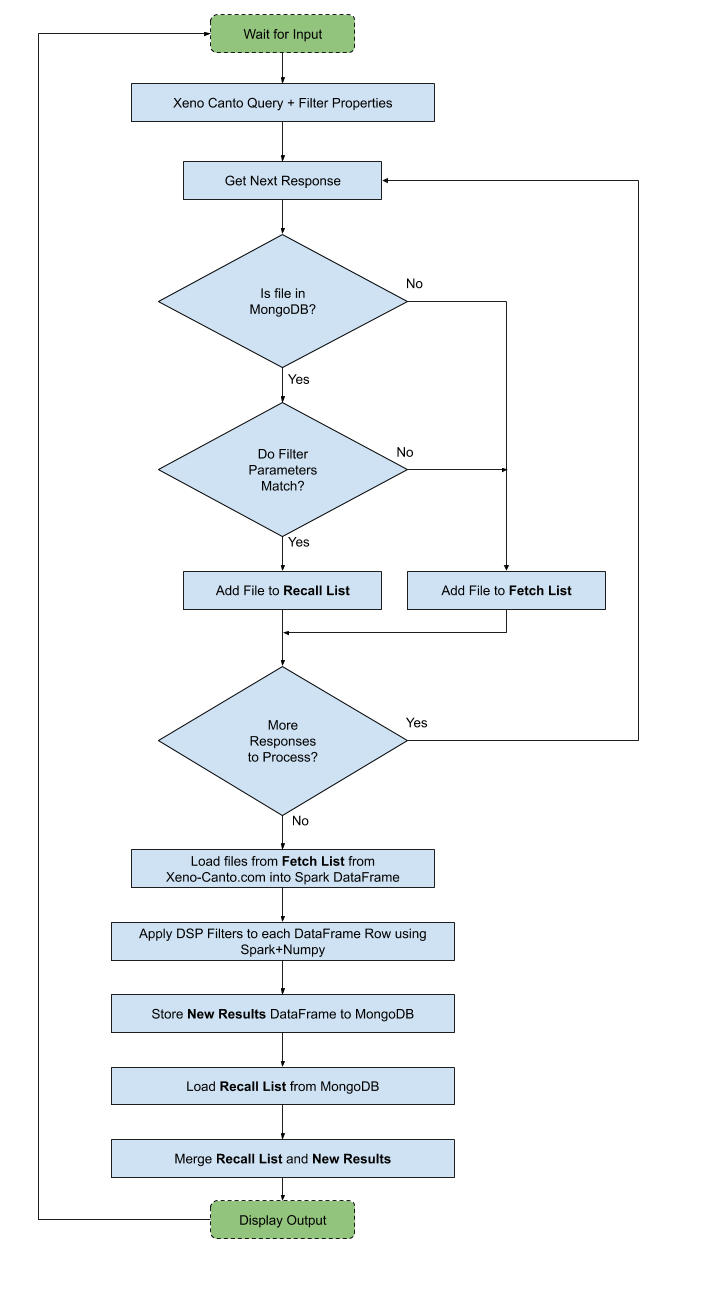
\includegraphics[width=3.4in]{project_flow_chart}
  \caption{Flow chart of the process used to merge querries from the cache and from the online database and then perform parallel processing using Apache Spark.}
  \label{fig:flow}
\end{figure}



\footnotetext{Our application is available at \url{https://github.com/MarkOfLark/gmu_ece_499_590_project} under the MIT License\cite{mitlicense} and subject to the George Mason University Honor Code\cite{gmuhonorcode}.}

%%%%%%%%%%%%%%%%%%%%%%%%%%%%%%%%%%%%%%%%%%%%%%%%%%%%%%%%%%%%%%%%%%%%%%%%%%%%%%%%%%%%%%%%%
%%%%%%%%%%%%%%%%%%%%%%%%%%%%%%%%%%%%%%%%%%%%%%%%%%%%%%%%%%%%%%%%%%%%%%%%%%%%%%%%%%%%%%%%%
%%%%%%%%%%%%%%%%%%%%%%%%%%%%%%%%%%%%%%%%%%%%%%%%%%%%%%%%%%%%%%%%%%%%%%%%%%%%%%%%%%%%%%%%%
%%%%%%%%%%%%%%%%%%%%%%%%%%%%%%%%%%%%%%%%%%%%%%%%%%%%%%%%%%%%%%%%%%%%%%%%%%%%%%%%%%%%%%%%%
\subsection{Caching the Xeno Canto Bird Call Database}
The \textit{xeno-canto} database has over 500,000 recordings from all around the world, generated by more than 6000 contributors, and representing close to 9000 hours of recordings\cite{xenocanto}. \textit{Xeno-canto} provides a rich API for querying the database which we used to populate the MongoDB database. These two technologies integrate seamlessly because the \textit{xeno-canto} API returns JSON data which directly forms the basis for documents in the MongoDB collection.

The example query in Listing \ref{lst:query}, which asks for all recordings made in the United States that are 10 seconds long ($\pm$ 1\%). It returns over 200 results, of which we use a subset for demonstration purposes.
\begin{lstlisting}[language=Txt, caption={\textit{Xeno-canto} Query}, label={lst:query}]
query=cnt:"united states"+len:10
\end{lstlisting}

Each result contains a host of metadata but for purposes of caching we are most interested in the \code{id} field which is a unique identifier provided by \textit{xeno-canto}.

We loop over each result and query MongoDB if an entry with a matching \code{id} is already in the file collection. We further query if an entry with a matching \code{id} has identical filter parameters to the parameters we requested. If it does not then we add this \code{id} to a list of recordings to be fetched and filtered. MongoDB's flexible schema allows for very straight forward matching of \code{id} fields and filter parameter fields which may or may not be present in each record, or of the same type and length. This is a desireable property since if a recording is present in the cache but was filtered with different parameters then we would still consider this a cache-miss.

After processing all of the results we have two lists of entries: recordings that were found in the cache and recordings that were not. We pass the list of not-found recordings to Spark through a Spark DataFrame for parallel downloading and processing.

%%%%%%%%%%%%%%%%%%%%%%%%%%%%%%%%%%%%%%%%%%%%%%%%%%%%%%%%%%%%%%%%%%%%%%%%%%%%%%%%%%%%%%%%%
%%%%%%%%%%%%%%%%%%%%%%%%%%%%%%%%%%%%%%%%%%%%%%%%%%%%%%%%%%%%%%%%%%%%%%%%%%%%%%%%%%%%%%%%%
%%%%%%%%%%%%%%%%%%%%%%%%%%%%%%%%%%%%%%%%%%%%%%%%%%%%%%%%%%%%%%%%%%%%%%%%%%%%%%%%%%%%%%%%%
%%%%%%%%%%%%%%%%%%%%%%%%%%%%%%%%%%%%%%%%%%%%%%%%%%%%%%%%%%%%%%%%%%%%%%%%%%%%%%%%%%%%%%%%%
\subsection{User Defined Functions}
Through the power of Apache Spark and the PySpark Python module we are able to download and process each recording in parallel. This capability is provided by the UDF (user defined function) module of PySpark. The signature of the UDF we defined for downloading and filtering is given in Listing \ref{lst:udf}.
\begin{lstlisting}[language=Txt, caption={PySpark User Defined Functions}, label={lst:udf}]
@udf(returnType=ArrayType(DoubleType()))
def load_and_filter(
  file_url,
  filter_edges,
  filter_amplitudes):
  ...
\end{lstlisting}
The annotation \code{@udf} tells PySpark that this function can be offloaded to the Spark engine and further that it should expect the return type to be an array of double precision values. This return type annotation is crucial since Spark is natively running the Scala programming language on the Java Virtual Machine so types of data that are transfered to the Spark engine must be mapped to Java language types.

To call this function we use the \code{select} operation on our DataFrame as shown in Listing \ref{lst:select}
\begin{lstlisting}[language=Txt, caption={PySpark DataFrame Select()}, label={lst:select}]
new_df = df.select(
  '*',
  load_and_filter(
    'file',
    'filter_edges',
    'filter_amplitudes').alias('file_content')
)
\end{lstlisting}
The \code{select} operation takes a comma-separated list of DataFrame column names and returns a new DataFrame with those columns. In this example we use \code{*} for the first parameter to say that we want to select all columns of the source DataFrame. The second parameter represents appending a new column to the DataFrame which will be called \code{file\_content} and will be the actual samples we read from the downloaded MP3 recording from \textit{xeno-canto} and filtered by our DSP filter. The source of this new column comes from three columns already in the DataFrame - \code{file}, \code{filter\_edges}, and \code{filter\_amplitudes} - that we pass to the UDF shown in Listing \ref{lst:udf}. The Spark engine will call this UDF on each row of the DataFrame in parallel using as many computing resources as are available in the Spark cluster. This means that downloading the original recording never occurs in the local processing environment.

%%%%%%%%%%%%%%%%%%%%%%%%%%%%%%%%%%%%%%%%%%%%%%%%%%%%%%%%%%%%%%%%%%%%%%%%%%%%%%%%%%%%%%%%%
%%%%%%%%%%%%%%%%%%%%%%%%%%%%%%%%%%%%%%%%%%%%%%%%%%%%%%%%%%%%%%%%%%%%%%%%%%%%%%%%%%%%%%%%%
%%%%%%%%%%%%%%%%%%%%%%%%%%%%%%%%%%%%%%%%%%%%%%%%%%%%%%%%%%%%%%%%%%%%%%%%%%%%%%%%%%%%%%%%%
%%%%%%%%%%%%%%%%%%%%%%%%%%%%%%%%%%%%%%%%%%%%%%%%%%%%%%%%%%%%%%%%%%%%%%%%%%%%%%%%%%%%%%%%%
\subsection{Digital Filtering}
After downloading a recording our UDF creates a digital filter using the Parks–McClellan algorithm\cite{dsp} according to the parameters specified by \code{filter\_edges} and \code{filter\_amplitudes}. This filter is then applied to the recording samples which are returned by the UDF and stored as a new column in the DataFrame called \code{file\_content} (as described in the previous section). It should be noted at this point that all the data movement (with the exception of the \textit{xeno-canto} metadata) has occured on the remote Spark cluster and not in the local Python environment.

%%%%%%%%%%%%%%%%%%%%%%%%%%%%%%%%%%%%%%%%%%%%%%%%%%%%%%%%%%%%%%%%%%%%%%%%%%%%%%%%%%%%%%%%%
%%%%%%%%%%%%%%%%%%%%%%%%%%%%%%%%%%%%%%%%%%%%%%%%%%%%%%%%%%%%%%%%%%%%%%%%%%%%%%%%%%%%%%%%%
%%%%%%%%%%%%%%%%%%%%%%%%%%%%%%%%%%%%%%%%%%%%%%%%%%%%%%%%%%%%%%%%%%%%%%%%%%%%%%%%%%%%%%%%%
%%%%%%%%%%%%%%%%%%%%%%%%%%%%%%%%%%%%%%%%%%%%%%%%%%%%%%%%%%%%%%%%%%%%%%%%%%%%%%%%%%%%%%%%%
\subsection{Merging New Results and Cached Results}
Merging new results and cached results is acomplished simply by creating a new Spark DataFrame from the Spark MongoDB connector plugin using a query of all requested \code{id} fields and not just the fields that required downloading and filtering. Since the last step performed by the UDF in listing \ref{lst:udf} is to store the new results DataFrame into MongoDB we can leverage MongoDB's ability to efficiently query documents and create a new Spark DataFrame that contains all the recordings we are interested in.

%%%%%%%%%%%%%%%%%%%%%%%%%%%%%%%%%%%%%%%%%%%%%%%%%%%%%%%%%%%%%%%%%%%%%%%%%%%%%%%%%%%%%%%%%
%%%%%%%%%%%%%%%%%%%%%%%%%%%%%%%%%%%%%%%%%%%%%%%%%%%%%%%%%%%%%%%%%%%%%%%%%%%%%%%%%%%%%%%%%
%%%%%%%%%%%%%%%%%%%%%%%%%%%%%%%%%%%%%%%%%%%%%%%%%%%%%%%%%%%%%%%%%%%%%%%%%%%%%%%%%%%%%%%%%
%%%%%%%%%%%%%%%%%%%%%%%%%%%%%%%%%%%%%%%%%%%%%%%%%%%%%%%%%%%%%%%%%%%%%%%%%%%%%%%%%%%%%%%%%
\subsection{Viewing Results}

\begin{figure*}  %image placeholder
  \centering
  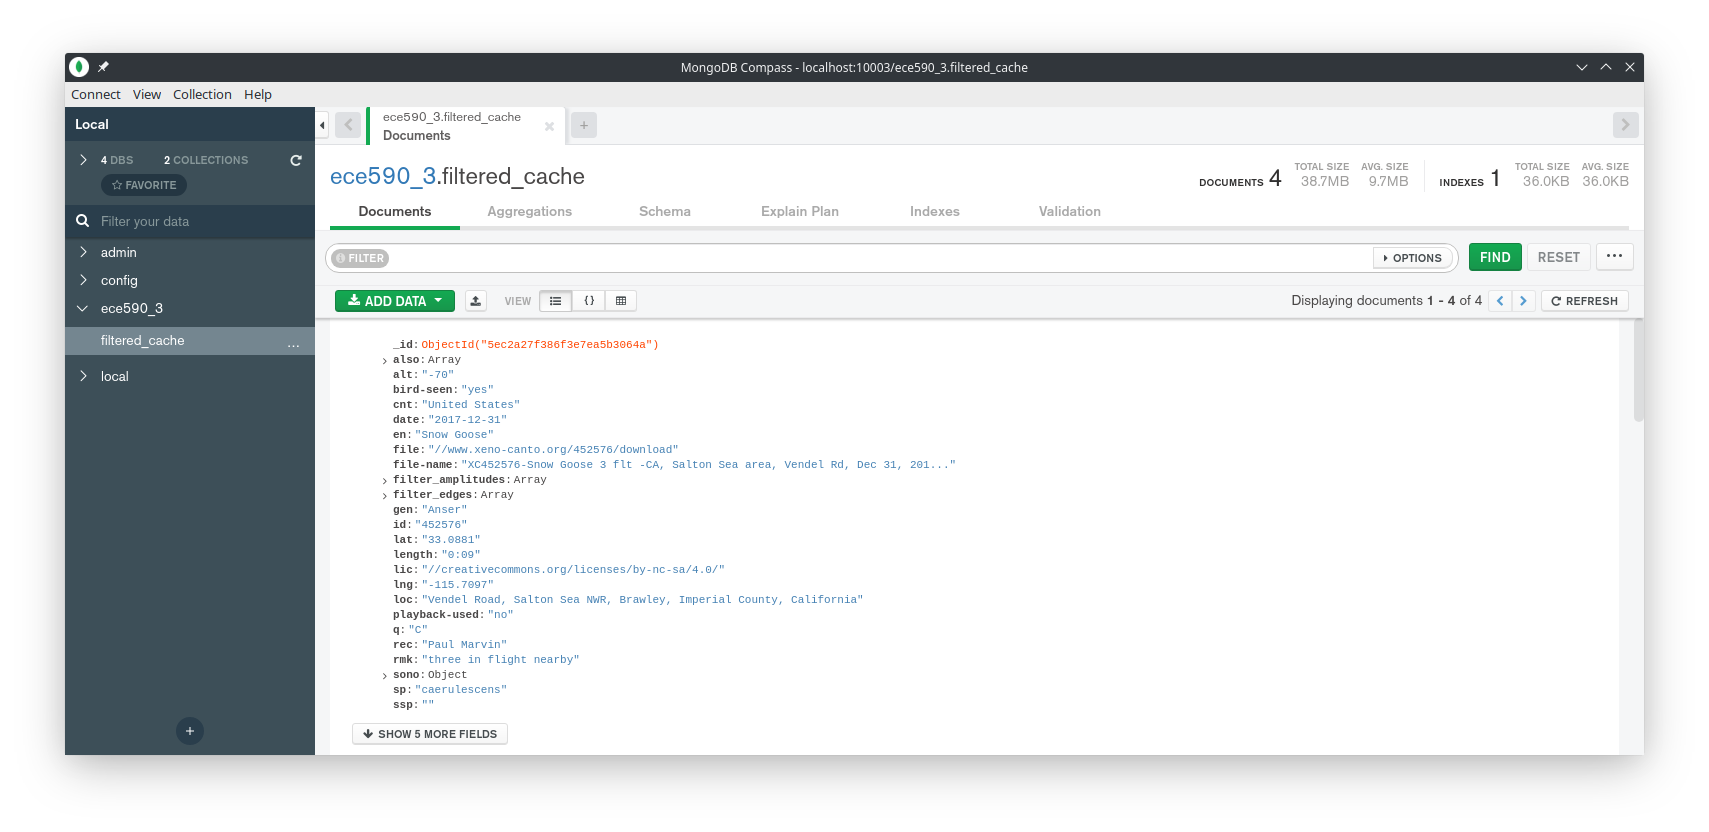
\includegraphics[width=\textwidth]{compass_screenshot}
  \caption{MongoDB Compass Application for viewing and managing MongoDB databases.}
  \label{fig:compass}
\end{figure*}


\begin{figure}
  \centering
  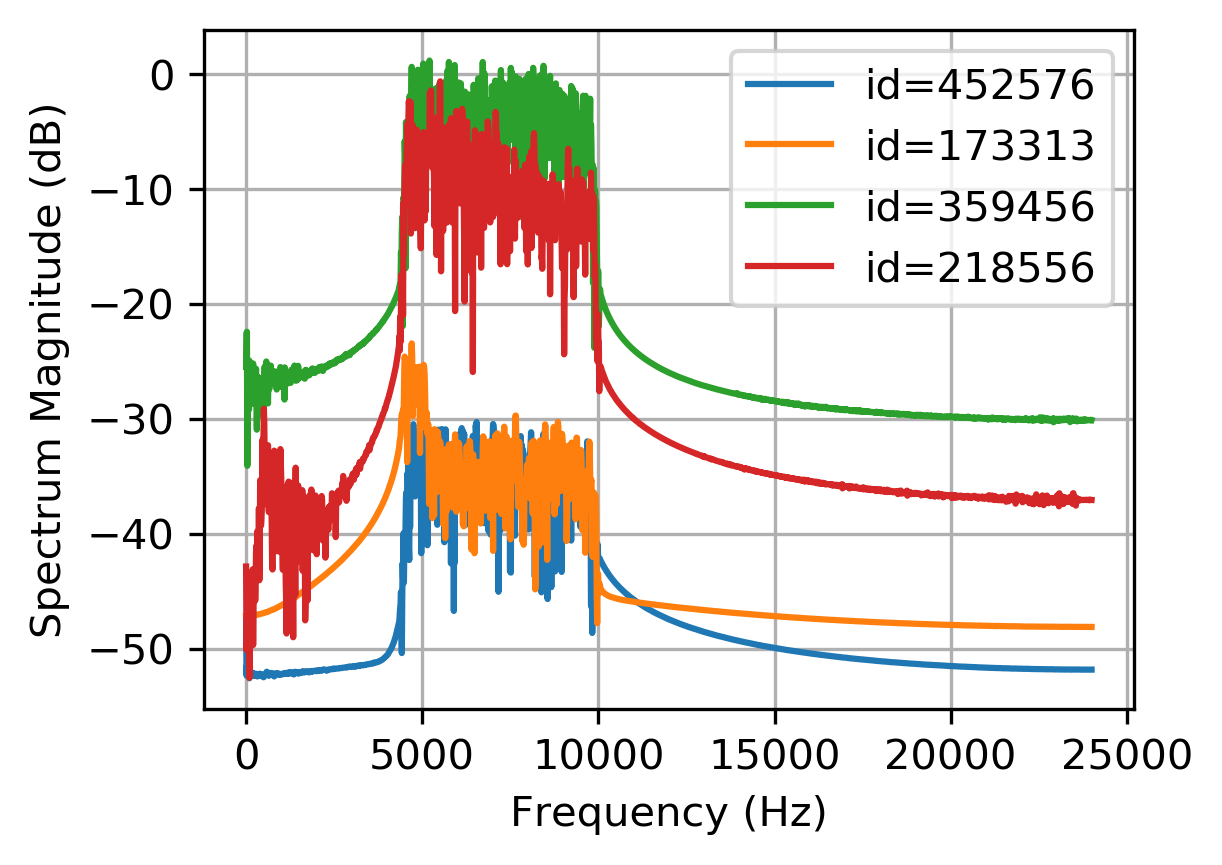
\includegraphics[width=3.4in]{output_spectrum}
  \caption{Results generated by running two separate Apache Spark jobs: one to download and apply a bandpass filter to four different recordings from xeno-canto.org in parallel, and another to compute the magnitude spectra of the recordings.}
  \label{fig:spectra}
\end{figure}

At this point we have a DataFrame where each row contains the results of filtering the \textit{xeno-canto} recordings. We could directly view these results by calling \code{collect} on the DataFrame but if we have more operations to perform it is more efficient to keep the data in Spark and offload further processing to the Spark cluster.

As an example of how to do this we created the UDF shown in Listing \ref{lst:spec}.
\begin{lstlisting}[language=Txt, caption={Taking FFTs with Spark}, label={lst:spec}]
@udf(returnType=ArrayType(DoubleType()))
def get_magnitude_spectrum( signal, Nfft ):
    return np.abs(
      np.fft.fft(
        np.array( signal ),
        n=Nfft
      )
    ).tolist()
\end{lstlisting}
Here we take the FFT of each signal and return that as a new column. To call this we again use the Spark DataFrame function \code{select} as shown in Listing \ref{lst:select2}. The difference from Listing \ref{lst:select} is that now we are not selecting all columns but only the columns we need since the result is going to get collected from the Spark cluster into our local python environment.
\begin{lstlisting}[language=Txt, caption={Collecting UDF Results for Local Processing}, label={lst:select2}]
Nfft = 4096
spec = df.select(
  'id',
  get_magnitude_spectrum(
    'file_content',
    lit(Nfft)
  ).alias('mag')
).collect()
\end{lstlisting}
The local DataFrame \code{spec} only contains the columns \code{id} and \code{mag}. For each row (there are 4 in this example) contains 4096 floating point values in the \code{mag} column which represents a huge reduction in memory since the original MP3 files were all approximately 10 seconds long with 48000 samples per second. Figure \ref{fig:spectra} shows local plots of the spectra for the 4 recordings that we fetched from the cache. Using Spark and UDFs we were able to obtain recordings, bandpass filter them, and obtain their spectra without ever moving data out of the Spark cluster until the last step. In this example we asked for filters that passed the band from 10\% to 20\% of the sampling frequency. We can see in the plot that we have indeed acheived the desired filtering.

Because the filtered files are cached in MongoDB, if we desire to visualize them in other ways or do further processing there is no need to download the source files again.

In addition to using Python data processing libraries (matplotlib, numpy) to visualize data we can also directly view and control the cache using MongoDB Compass\cite{mongodbcompass} as described before. Figure \ref{fig:compass} shows one of the cache entries visualized by that tool.

%%%%%%%%%%%%%%%%%%%%%%%%%%%%%%%%%%%%%%%%%%%%%%%%%%%%%%%%%%%%%%%%%%%%%%%%%%%%%%%%%%%%%%%%%
%%%%%%%%%%%%%%%%%%%%%%%%%%%%%%%%%%%%%%%%%%%%%%%%%%%%%%%%%%%%%%%%%%%%%%%%%%%%%%%%%%%%%%%%%
%%%%%%%%%%%%%%%%%%%%%%%%%%%%%%%%%%%%%%%%%%%%%%%%%%%%%%%%%%%%%%%%%%%%%%%%%%%%%%%%%%%%%%%%%
%%%%%%%%%%%%%%%%%%%%%%%%%%%%%%%%%%%%%%%%%%%%%%%%%%%%%%%%%%%%%%%%%%%%%%%%%%%%%%%%%%%%%%%%%
%%%%%%%%%%%%%%%%%%%%%%%%%%%%%%%%%%%%%%%%%%%%%%%%%%%%%%%%%%%%%%%%%%%%%%%%%%%%%%%%%%%%%%%%%
%%%%%%%%%%%%%%%%%%%%%%%%%%%%%%%%%%%%%%%%%%%%%%%%%%%%%%%%%%%%%%%%%%%%%%%%%%%%%%%%%%%%%%%%%
%%%%%%%%%%%%%%%%%%%%%%%%%%%%%%%%%%%%%%%%%%%%%%%%%%%%%%%%%%%%%%%%%%%%%%%%%%%%%%%%%%%%%%%%%
%%%%%%%%%%%%%%%%%%%%%%%%%%%%%%%%%%%%%%%%%%%%%%%%%%%%%%%%%%%%%%%%%%%%%%%%%%%%%%%%%%%%%%%%%
\section{Conclusion}
In conclusion based on the projects result we can conclude that in fact the project operated as intended as seen in the data and graphs in the report. The scope of this project was to incorporate the techniques learned in ECE 499 and combine those techniques with Machine Learning and signal processing. Although this was just incorporated in something as simple as bird sounds these practices can be scaled onto data that is more rigorous and/or import. Finally this report hopes to inform the audience of the bridge between Signal Processing and Machine Learning and how they can be applied to uses cases.


% \footnotetext{The implementation is available upon request under the MIT Open Source Software license and subject to the George Mason University Honor Code.}

% if have a single appendix:
%\appendix[Implementation]
%My implementation is available upon request under the MIT Open Source Software license.
% or
%\appendix  % for no appendix heading
% do not use \section anymore after \appendix, only \section*
% is possibly needed

% use appendices with more than one appendix
% then use \section to start each appendix
% you must declare a \section before using any
% \subsection or using \label (\appendices by itself
% starts a section numbered zero.)
%


%\appendices
%\section{Proof of the First Zonklar Equation}
%Appendix one text goes here. \cite{MRABF}

% you can choose not to have a title for an appendix
% if you want by leaving the argument blank
%\section{}
%Appendix two text goes here.


% use section* for acknowledgment
%\section*{Acknowledgment}
%The authors would like to thank...


% Can use something like this to put references on a page
% by themselves when using endfloat and the captionsoff option.
\ifCLASSOPTIONcaptionsoff
  \newpage
\fi



% trigger a \newpage just before the given reference
% number - used to balance the columns on the last page
% adjust value as needed - may need to be readjusted if
% the document is modified later
%\IEEEtriggeratref{8}
% The "triggered" command can be changed if desired:
%\IEEEtriggercmd{\enlargethispage{-5in}}

% references section

% can use a bibliography generated by BibTeX as a .bbl file
% BibTeX documentation can be easily obtained at:
% http://mirror.ctan.org/biblio/bibtex/contrib/doc/
% The IEEEtran BibTeX style support page is at:
% http://www.michaelshell.org/tex/ieeetran/bibtex/
\bibliographystyle{IEEEtran}
% argument is your BibTeX string definitions and bibliography database(s)
\bibliography{IEEEabrv,project}
%
% <OR> manually copy in the resultant .bbl file
% set second argument of \begin to the number of references
% (used to reserve space for the reference number labels box)
%\begin{thebibliography}{1}

%\bibitem{IEEEhowto:kopka}
%H.~Kopka and P.~W. Daly, \emph{A Guide to \LaTeX}, 3rd~ed.\hskip 1em plus
%  0.5em minus 0.4em\relax Harlow, England: Addison-Wesley, 1999.

%\end{thebibliography}

% biography section
%
% If you have an EPS/PDF photo (graphicx package needed) extra braces are
% needed around the contents of the optional argument to biography to prevent
% the LaTeX parser from getting confused when it sees the complicated
% \includegraphics command within an optional argument. (You could create
% your own custom macro containing the \includegraphics command to make things
% simpler here.)
%\begin{IEEEbiography}[{\includegraphics[width=1in,height=1.25in,clip,keepaspectratio]{mshell}}]{Michael Shell}
% or if you just want to reserve a space for a photo:

%\begin{IEEEbiography}{Michael Shell}
%Biography text here.
%\end{IEEEbiography}

% if you will not have a photo at all:
%\begin{IEEEbiographynophoto}{John Doe}
%Biography text here.
%\end{IEEEbiographynophoto}

% insert where needed to balance the two columns on the last page with
% biographies
%\newpage

%\begin{IEEEbiographynophoto}{Jane Doe}
%Biography text here.
%\end{IEEEbiographynophoto}

% You can push biographies down or up by placing
% a \vfill before or after them. The appropriate
% use of \vfill depends on what kind of text is
% on the last page and whether or not the columns
% are being equalized.

%\vfill

% Can be used to pull up biographies so that the bottom of the last one
% is flush with the other column.
%\enlargethispage{-5in}



% that's all folks
\end{document}


